
\subsection{Rules \texorpdfstring{$R_{LR}$}{RLR}: from  LA to RA and Back}
In this section we describe our approach of optimizing LA expressions
by converting them to RA.  The rules converting from LA to RA and back
are denoted $R_{LR}$.

To justify our approach, let us revisit our example loss function
written in LA and attempt to optimize it using standard LA identities.
Here we focus on algebraic rewrites and put aside concerns about the
cost model. Using the usual identities on linear algebra expressions,
one may attempt to rewrite the original expression as follows:
\begin{align*}
& sum((X-UV^T)^2) \\
= &sum((X-UV^T)*(X-UV^T)) \\
=&sum(X^2-2X*UV^T+(UV^T)^2) \\
= & sum(X^2) - 2sum(X*UV^T) + sum((UV^T)^2)
\end{align*}
% \dan{$(UV^T)^2$ should be $sum(UV^T)^2$.}
At this point we are stuck trying to rewrite $sum(X*UV^T)$ (recall
that $*$ is element-wise multiplication); it turns out to be equal to
$sum(U^TXV)$, for any matrices $X,U,V$ (and it is equal to the scalar
$U^TXV$ when $U, V$ are column vectors), but this does not seem to
follow from standard LA identities like associativity, commutativity,
and distributivity.  Similarly, we are stuck trying to rewrite
$sum((UV^T)^2)$ to $sum(U^TU * V^TV)$.  Current systems manually add
syntactic rewrite rules, whenever such a special case is deemed
frequent enough to justify extending the optimizer.


\begin{figure}
\centering
%%% (Dan: I replaced the multiplicies 1,2 with different ones so
%%% readers don't confuse them with indices in the matrix)
\begin{tabular}{ccccc}
&
     $A$ & $x$ & $A * x^T$ & $Ax$\\
     \hline
     \\[-1em]
LA: &
     $\begin{bmatrix}
    0 & 5 \\
    7 & 0
    \end{bmatrix}$ & $\begin{bmatrix}
    3\\
    2
    \end{bmatrix}$ & $\begin{bmatrix}
    0 & 10 \\
    21 & 0
    \end{bmatrix}$ & $\begin{bmatrix}
    10 \\
    21
    \end{bmatrix}$ \\
    \\[-0.8em]
    \hline
RA: &
    \begin{tabular}{|c|c|c}
    $i$ &$j$&\# \\
    \hline
        $1$ & $2$ & 5 \\
        $2$ & $1$ & 7
    \end{tabular}{} &
    \begin{tabular}{|c|c}
         $j$ &\# \\
         \hline
         1 & 3\\
         2 & 2
    \end{tabular}{} &
    \begin{tabular}{|c|c|c}
    $i$ &$j$ & \# \\
    \hline
        $1$ & $2$ & 10 \\
        $2$ & $1$ & 21
    \end{tabular}{} &
    \begin{tabular}{|c|c}
         $i$ & \# \\
         \hline
         1 & 10 \\
         2 & 21
    \end{tabular}{} 
    
\end{tabular}{}
    
\caption{Top: Linear Algebra manipulates matrices and vectors.
  $A*x^T$ is element-wise multiplication, computing the matrix
  $(A_{ij}x_j)_{ij}$, while $Ax$ is standard matrix-vector
  multiplication.  Bottom: their translations into $K$-relations and
  Relational Algebra operations.  Each relation is a bag, where the
  attribute $\#$ represents the multiplicity, i.e. $A(1,2)$ has
  multiplicity $5$ etc.  Then $A*x^T$ becomes a standard query
  $Q(i,j) = A(i,j)*x(j)$, while $Ax$ is a query with a group-by and
  aggregate, $Q(i) = \sum_j A(i,j)*x(j)$.}
    \label{matrixkrel}
\end{figure}{}

Instead, our approach is to expand out the LA expression element-wise.
For example, assuming for simplicity that $U,V$ are column vectors, we
obtain
\begin{align*}
& sum((UV^T)^2) = \textstyle{\sum_{i,j}} (U_i * V_j) * (U_i * V_j) \\
& = \textstyle{\sum_{i,j}}(U_i * U_i) * (V_j * V_J) \\
& = ( \textstyle{\sum_i} U_i * U_i) * ( \textstyle{\sum_j} V_j * V_j)  \\
& = U^TU * V^TV
\end{align*}
%
The expressions using indices represent Relational Algebra
expressions.  More precisely, we interpret every vector, or matrix, or
tensor, as a $K$-relation~\cite{DBLP:conf/pods/GreenKT07} over the
reals. In other words we view $X_{ij}$ is a tuple $X(i,j)$ whose
``multiplicity'' is the real value of that matrix element.  We
interpret point-wise multiply as natural join; addition as union; sum
as aggregate; and matrix multiply as aggregate over a join\footnote{In
  the implementation, we use outer join for point-wise multiply and
  addition, where we multiply and add the matrix entries
  accordingly. In this paper we use join and union to simplify
  presentation.}.
%
Figure~\ref{matrixkrel} illustrates the correspondence between LA and
RA.  We treat each matrix entry $A_{ij}$ as the multiplicity of tuple
$(i, j)$ in relation $A$ under bag semantics. For example
$A_{2,1} = 7$, therefore the tuple $(2,1)$ has multiplicity of $7$ in
the corresponding relation.  $A*x^T$ denotes element-wise
multiplication, where each element $A_{ij}$ of the matrix is
multiplied with the element $x_j$ of the row-vector $x^T$.  In RA it
is naturally interpreted as the natural join $A(i,j) \Join x(j)$,
which we write as $A(i,j)*x(j)$.  Similarly, $Ax$ is the standard
matrix-vector multiplication in LA, while in RA it becomes a query
with a group by and aggregate, which we write as $\sum_j A(i,j)*x(j)$.
Our $K$-relations are more general than bags, since the entry of a
matrix can be a real number, or a negative number; they correspond to
$K$-relations over the semiring of reals $(\R, 0, 1, +, *)$.

% Of course, a matrix can have an entry that is not an integer, which
% would not make sense as multiplicity. In general, the matrix entries
% corresponds to the semiring of reals which serve as relation
% annotations \cite{DBLP:conf/pods/GreenKT07} in the $K$-relation.
\begin{table}
\centering
\begin{tabular}{llll}
&name & type & syntax \\ \hline \multirow{7}{*}{\rotatebox[origin=c]{90}{LA}}
  &mmult & $M_{M,L} \times M_{L,N} \rightarrow M_{M,N}$ & $AB$ or MxM
  \\ &elemmult & $M_{M,N} \times M_{M,N} \rightarrow M_{M,N}$ & $A*B$
  \\ &elemplus & $M_{M,N} \times M_{M,N} \rightarrow M_{M,N}$ & $A+B$ \\ &rowagg
  & $M_{M,N} \rightarrow M_{M,1}$ & $sum_{row} A$ \\ &colagg & $M_{M,N}
  \rightarrow M_{1,N}$ & $sum_{col} A$ \\ &agg & $M_{M,N} \rightarrow M_{1,1}$ &
  $sum A$ \\
%&power & $M  \times Int \rightarrow M$ & $A^k$ \\
&transpose & $M_{M,N} \rightarrow M_{N,M}$ & $A^\tr$ \\ \hline
  \multirow{2}{*}{\rotatebox[origin=c]{90}{conv.}} &bind & $M_{M,N} \times [i,j]
  \rightarrow R_{i:M,j:N}$ & $\bind{i,j} A$ \\ &unbind & $R_{i:M,j:N} \times
              [i,j] \rightarrow M_{M,N}$ & $\unbind{i}{j} A$ \\ \hline
              \multirow{2}{*}{\rotatebox[origin=c]{90}{RA}} &join & $R_{S_1}
              \times R_{S_2} \rightarrow R_{S_1 \cup S_2}$ & $A \rmul B$
              \\ &union & $R_{S_1} \times R_{S_2} \rightarrow R_{S_1 \cup S_2}$
              & $A \radd B$ \\ &agg & $R_S \times U \rightarrow R_{S \setminus
                U}$ & $\sum_{U} A$ \\
\end{tabular}
\caption{LA and RA Operators. The type $M_{M,N}$ is a matrix of size $M \times
  N$; $[i,j]$ is a list of attribute names; $R_{i:M,j:N}$ is a relation with
  attributes $i$ of size $M$ and $j$ of size $N$; $S_1, S_2, S,$ and $U$ are
  sets of attributes.}
\label{tPlanOps}
\end{table}
\begin{figure}
\centering
\begin{minipage}{0.6\textwidth}
\begin{enumerate}
  \item $A*B \rightarrow \unbind{i}{j}(\bind{i,j}A \rmul \bind{i,j}B)$.
  \item $A+B \rightarrow \unbind{i}{j}(\bind{i,j}A \radd \bind{i,j}B)$.
  \item $sum_{row} A \rightarrow [-i,\_ ] \sum_j \bind{i,j} A$. Similar for
    $sum_{col}$, $sum$.
  \item $AB \rightarrow \unbind{i}{k} \sum_j (\bind{i,j}A \rmul \bind{j,k}B)$.
  \item $A^\tr \rightarrow \unbind{j}{i} \bind{i,j}A$.
  \item $A - B \rightarrow A + (-1) * B$
\end{enumerate}
\end{minipage}{}
\caption{LA-to-RA Ruleset $R_{LR}$. Notice that $*$ means point-wise multiply for matrices,
  but means natural join for relations. Similarly, $+$ means addition for matrices, but
  union for relations.}
\label{RMR}
\end{figure}

% Following our relational semantics, $sum((X-UV^T)^2)$ is interpreted
% as
% $\sum_{ij} (X_{ij} - U_{i} \bowtie V_{j}) \bowtie (X_{ij} - U_{i}
% \bowtie V_{j})$. Note that because $U$ and $V$ are vectors, the
% aggregate in their matrix product $\sum_{\varnothing} U_i \bowtie V_j$
% is over an empty set of attributes and therefore eliminated.
% Hereafter we will overload $*$ for join and $+$ for union to keep our
% formulas intuitive.  Table~\ref{tPlanOps} provides the list of LA and
% RA operators.  

We now describe the general approach in \sys.  The formal definition
of LA and RA are in Table~\ref{tPlanOps}.  LA consists of seven
operators, which are those supported in
SystemML~\cite{DBLP:reference/bdt/Boehm19}.  RA consists of only three
operators: $*$ (natural join), $+$ (union), and $\sum$ (group-by
aggregate).  Difference is represented as $A-B = A + (-1)B$ (this is
difference in $\R$; we do not support bag difference, i.e.  difference
in $\N$ like $3-5=0$, because there is no corresponding operation in
LA), while selection can be encoded by multiplication with relations
with 0/1 entries.  We call an expression using these three RA
operators an {\em RPlan}, for Relational Plan, and use the terms RPlan
and RA/relational algebra interchangeably.  Finally, there are two
operators, {\em bind} and {\em unbind} for converting between
matrices/vectors and $K$-relations.


The translation from LA to RA is achieved by a set of rules, denoted
$R_{LR}$, and shown in Figure~\ref{RMR}. The bind operator
$\bind{i,j}$ converts a matrix to a relation by giving attributes
$i,j$ to its two dimensions; the unbind operator $\unbind{i}{j}$
converts a relation back to a matrix. For example,
$\unbind{j}{i}\bind{i,j}A$ binds $A$'s row indices to $i$ and its
column indices to $j$, then unbinds them in the opposite order,
thereby transposing $A$.

\sys\ translates a complex LA expression into RA by first applying the
rules $R_{LR}$ in Figure~\ref{RMR} to each LA operator, replacing it
with an RA operator, preceded by {\em bind} and followed by {\em
  unbind}. Next, it eliminates consecutive unbind/bind operators,
possibly renaming attributes, e.g.  $\bind{k,l} \unbind{i}{j} A$
becomes $A[i \to k, j \to l]$, which indicates that the attributes $i$
and $j$ in $A$'s schema should be renamed to $k$ and $l$, by
propagating the rename downward into $A$.  As a result, the entire LA
expression becomes an RA expression (RPlan), with {\em bind} operators
on the leaves, and {\em unbind} at the top.
% The result of eliminating unbind and bind operators is an RA
% expression with a bind operator above every (nonscalar) input and an
% unbind operator below every (nonscalar) output.
For an illustration, the left DAG in Figure~\ref{fig:radags} shows the
expression $sum((X - UV^T)^2)$ translated to relational algebra.

\begin{figure}
\centering
\begin{minipage}{0.6\textwidth}
\begin{enumerate}
  \item\label{RRC_mp} $A \rmul (B \radd C) = A \rmul B \radd A \rmul C$
  \item\label{RRC_ap} $\sum_i (A \radd B) = \sum_i A \radd \sum_i B$
  \item\label{RRC_ma} If $i \not\in A$, $A \rmul \sum_i B = \sum_i (A \rmul B)
    \quad$ (else rename $i$)
  \item\label{RRC_aa} $\sum_i \sum_j A = \sum_{i,j} A$
%   \item $\sum_i A \rightarrow \sum_{i,j} A$
  \item\label{RRC_ac} If $i \not\in Attr(A)$, then $\sum_i A = A \rmul dim(i)$
  \item\label{RRC_pp} $A \radd (B \radd C) = +(A, B, C) \quad$ (assoc. \& comm.)
  \item\label{RRC_mm} $A \rmul (B \rmul C) = *(A, B, C) \quad$ (assoc. \& comm.)
\end{enumerate}
\end{minipage}
\caption{RA equality rules $R_{EQ}$. $*$ means natural join and $+$ means
  union.}
\label{RRC}
\end{figure}


\begin{figure}
    \centering
    
\includegraphics[width=0.6\linewidth]{wormhole}
    \caption{Venn diagram of LA and/or RA expressions.  Each of the two
      white islands represent LA expressions that can be proven
      equivalent using identities in LA; there is no way to move from
      one island to the other by using LA identities.  The large gray
      box shows the set of expressions that can be proven equivalent
      by using RA identities.  This allows us to connect the two
      islands. }
    \label{wormhole}
\end{figure}{}
\begin{figure}
    \centering
\begin{tikzcd}
e_{LA} \arrow[rr, "=" description, no head, dotted] \arrow[d, "R_{LR}"'] &           & e'_{LA} \arrow[d, "R_{LR}"]  \\
e_{RA} \arrow[r, "R_{EQ}"]                                               & \mathcal{C}(e_{RA}) \equiv \mathcal{C}(e'_{RA})  & e'_{RA} \arrow[l, "R_{EQ}"']
\end{tikzcd}
    
    \caption{Two LA expressions $e_{LA}$ and $e'_{LA}$ are equivalent \textit{iff} their
    relational counterparts $e_{RA}$ and $e'_{RA}$ have isomorphic
      canonical forms $\mathcal{C}(e_{RA}), \mathcal{C}(e'_{RA})$. $R_{LR}$ translates a LA expression to RA and $R_{EQ}$ are the relational equality rules. }
    \label{proofsketch}
\end{figure}{}

\begin{figure}
    \centering
    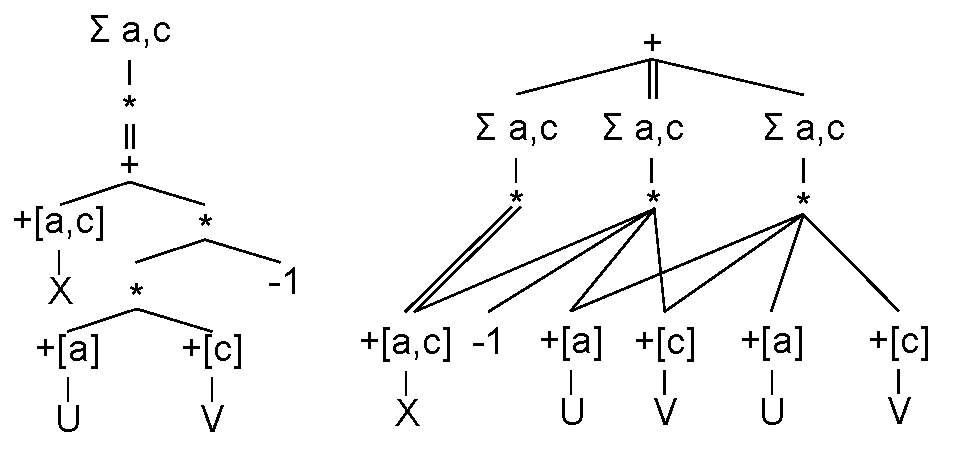
\includegraphics[width=0.6\linewidth]{img/radags.pdf}
    \caption{RA DAGs for $sum((X-UV^T)^2)$ (left) and its canonical form (right). }
    \label{fig:radags}
\end{figure}{}

% \begin{figure*}
%     \centering 
\includegraphics[width=\textwidth]{parrot}
%     \caption{Rewriting details using $R_{LR}$ and $R_{EQ}$ and the
%       optimization's impact on execution cost. Here we show the general case
%       where $U$ and $V$ are matrices, and $X*UV^T$ is computed with a fused
%       chain multiplication operator that exploits sparsity. Dashed lines
%       highlight the initial RPlan and its canonical form. }
%     \label{parrot}
% \end{figure*}




\subsection{Rules \texorpdfstring{$R_{EQ}$}{REQ} : from RA to RA}\label{sec:req}

The equational rules for RA consists of seven identities shown in
Figure~\ref{RRC}, and denoted by $R_{EQ}$.  The seven rules are
natural relational algebra identities, where $*$ corresponds to
natural join, $+$ to union (of relations with the same schema) and
$\sum_i$ to group-by and aggregate.  In rule~\ref{RRC_ac},
$i \notin Attr(A)$ means that $i$ is not an attribute of $A$, and
$dim(i)$ is the dimension of index $i$.  For a very simple
illustration of this rule, consider $\sum_i 5$.  Here $5$ is a
constant, i.e. a relation of zero arity, with no attributes.  The rule
rewrites it to $5 dim(i)$, where $dim(i)$ is a number representing the
dimension of $i$.

%%% (Dan: I think the example below is wrong. In RA you must have
%%% indices, can't write $x+1$.
%  $\sum_i (x + 1)$ where $x$ is a vector of length 10 and
% $x + 1$ adds $1$ with each entry of $x$. Following rule~\ref{RRC_ap},
% pushing down the summation rewrites the expression to
% $\sum_i x + \sum_i 1$, and now rule~\ref{RRC_ac} rewrites $\sum_i 1$
% to $|i| * 1 = 10$.


\subsection{Completeness of the Optimization Rules}\label{ranf}

As we have seen at the beginning of this section, when rewriting LA
expressions using identities in linear algebra we may get stuck.  This
is illustrated in Figure~\ref{wormhole}, which shows two white islands
representing sets of provably equivalent LA expressions; the simple
identities in LA allow us to move within one white island, but are
insufficient to move from one island to the other.  Instead, by
rewriting the expressions to RA, the seven identities in $R_{EQ}$ are
much more powerful, and allow us to prove them equivalent.  We prove
here that this approach is {\em complete}, meaning that, if two LA
expressions are semantically equivalent, then their equivalence can be
proven by using rules $R_{EQ}$.  The proof consists of two parts: (1)
the rules $R_{EQ}$ are sufficient to convert any RA expression $e$ to
its {\em normal form} (also called {\em canonical form})
$\mathcal{C}(e)$, and back, (2) two RA expressions $e, e'$ are
semantically equal iff they have isomorphic normal forms,
$\mathcal{C}(e) \equiv \mathcal{C}(e')$.
% 
% 
% 
% In general, any equivalent LA expressions can be rewritten to each other using
% our RA representation and equalities. In other words, the relational equalities
% $R_{EQ}$ are \textit{complete} w.r.t. linear algebra semantics. For
% optimization, this means RPlan and its equalities completely represent the
% search space of the optimization problem: we can rewrite an LA expression to any
% of its equals if we first translate it into RA, then apply a chain of equalities
% from $R_{EQ}$, and finally translate the result back to LA. As
% Figure~\ref{wormhole} illustrates, while the usual linear algebra identities
% $R_{LA}$ can only create disjoint equality space for our example expression pre-
% and post-optimization, the relational rules connects the space and rewrite the
% slow expression to the fast one. We sketch a proof of completeness in this
% section.
% 
Figure~\ref{proofsketch} shows the main steps at a high level: two LA
expressions are semantically equivalent if and only if their canonical
form in RA are isomorphic, where $R_{LR}$ translates each expression
to RA and $R_{EQ}$ takes the RA expression to its canonical form.
Throughout this section we write $e\ R_{EQ}^*\ e'$ when $e, e'$ can be
proven equal by using the identities in $R_{EQ}$ (Fig.~\ref{RRC}).

% By semantically equivalent, we
% mean two expressions evaluate to the same result given any same input (variable
% assignment). We define isomorphism of RA canonical forms in Section~\ref{ranf}.

{\bf Normal Form} The normal form of an RPlan is similar in spirit to
the canonical form of polynomials as a sum of monomials, except that
the monomial terms also include aggregations.  As for polynomials, we
combine equal factors by introducing power, e.g. $X * X$ becomes
$X^2$, and combine isomorphic monomials by introducing constant
coefficients, e.g. $3X^2Y+5X^2Y$ becomes $8X^2Y$.  For example, the
following RPlan denotes a 1-dimensional vector
$Q(i) = (\sum_j x(i,j) * (\sum_k y(j,k)*x(i,j)) + \sum_{m,n} x(i,m)^2
y(m,n)$ and its canonical form is $2 \sum_{j,k} x(i,j)^2y(j,k)$.
Formally:

% 
% 
% Polynomials in their
% canonical form may not be the most efficient form to execute, but they
% do act as a canonical form and also serve as a starting point for
% finding more efficient forms. The analogy to polynomials extends
% further: the canonical form of polynomials combines \textit{like
%   terms}, i.e., two terms that have the same variables. Instead of
% writing $3X^2Y + 5X^2Y$, for example, we write its canonical form as
% $8X^2Y$. For RA expressions, we determine whether two terms are like
% by whether there exists an isomorphism mapping one to the other by
% renaming attributes (up to a constant scalar).
% 
% The canonical form for RA expressions is the sum-of-aggregations-of-products
% with like terms combined, as follows:

\begin{definition}
  An RA expression is \textbf{canonical}, or in \textbf{normal form},
  if it is the sum (i.e. $+$) of $n$ {\em monomials}, where each
  monomial $i$ consists of a constant $c_i$ multiplied by an
  aggregation over a (possibly empty) set of attributes $A_i$ (for
  $1 \leq i \leq n$), of a product of $m_i$ {\em factors}, where each
  factor is some matrix or vector $x_{ij}$ (for $1 \leq i \leq n$,
  $1 \leq j \leq m_i$) indexed by some index variables (not shown),
  and possibly raised to some power:

\[c_1 \sum_{A_1} \lrparen{x_{11}^{k_{11}} * \dots * x_{1m_1}^{k_{1m_1}}} %+ \sum_{A_2} (b_{21} * \dots * b_{2m_2})
+ \dots + c_n \sum_{A_n} \lrparen{x_{n1}^{k_{n1}} * \dots * x_{nm_n}^{k_{nm_n}}}\]

We further assume that no monomial contains the same factor twice
(otherwise, replace it with a single factor with a higher power
$k_{ij}$) and no two monomials are isomorphic (otherwise we replace
them with a single monomial with a larger coefficient $c_i$)
% 
% Further, there must not exist, for any $1 \leq i < j \leq n$, an isomorphism
% $\phi$ renaming attributes in the schema of $b_{i1} * \dots * b_{im_i}$ to
% attributes in the schema of $b_{j1} * \dots * b_{jm_j}$ such that $m_i=m_j$,
% $\phi(A_i) = A_j$, and $\phi\{b_{i1} * \dots * b_{im_i}\} = \{b_{j1} * \dots *
% b_{jm_j}\}$.
% 
\end{definition}
The order of summands and multiplicands is insignificant because $*$
and $+$ are commutative and associative.  We notice that, unlike
traditional polynomials, here the same matrix name may occur in
different factors, for example in $\sum_{i,j,k} x(i,j)*x(j,k)*x(k,i)$
the matrix $x$ occurs three times, but the factors are different
i.e. we cannot write $x^3$.

The first of the completeness proof consists in showing that every
expression $e$ in RA is equivalent to some normal form
$\mathcal{C}(e)$, and, moreover, that their equivalence can be proven
using the rules $R_{EQ}$ in Figure~\ref{RRC}.

\begin{lemma}\label{lCanonPreservesSemantics}
$\forall e \in RA$ there exists a canonical form $\mathcal{C}(e)$ and,
moreover, their equivalence follows from the rules in $R_{EQ}$, in
notation: $e\ R_{EQ}^*\  \mathcal{C}(e)$.
\end{lemma}

The proof is a straightforward induction on the structure of $e$.  We
apply distributivity of $*$ over $+$, then pull out the summation
$\sum$; we omit the details.  We illustrate in Figure~\ref{fig:radags}
the canonical form of the expression $sum((X-UV^T)^2)$.  Notice that,
since the rules in $R_{EQ}$ are sound, it follows that any expression
$e$ has {\em the same semantics} as its canonical form
$\mathit{C}(e)$.

%  and its
% canonical form. Let $\mathcal{C}$ be the transitive application of
% ruleset $R_{EQ}$, replacing any expression matching the left hand side
% of a rule by the expression on the right hand side. The following
% properties of $\mathcal{C}$ show it truly is canonicalizing.
% 


%% \begin{proof}
%% 
%% 
%% 
%% 
%% By structural induction over $p$.
%% % Proceed by structural induction over an RA expression $p$. The base case, that
%% % $p$ is a lone relation, is canonical. The inductive cases are as follows.
%% % 1) Suppose $p = p^1 + p^2$. By the inductive hypothesis, $p^1$ and $p^2$ are
%% % canonical with forms, for $i \in \{1,2\}$, \\ $\sum_{A^i_{1}} \lrparen{b^i_{11}
%% %   * \dots * b^i_{1m^i_{1}}} + \dots + \sum_{A^i_{n^i}} \lrparen{b^i_{n^i1} *
%% %   \dots * b^i_{n^im^i_{n^i}}}$.
%% % By rule~\ref{RRC_pp}, $p$ takes the canonical form \\ $\sum_{A^1_{1}}
%% % \lrparen{b^1_{11} * \dots * b^1_{1m^1_{1}}} + \dots + \sum{A^1_{n^1}}
%% % \lrparen{b^1_{n^11} * \dots * b^1_{n^1m^1_{n^1}}} + \sum_{A^2_{1}}
%% % \lrparen{b^2_{11} * \dots * b^2_{1m^2_{1}}} + \dots + \sum{A^2_{n^2}}
%% % \lrparen{b^2_{n^21} * \dots * b^2_{n^2m^2_{n^2}}}$.
%% % 2) Suppose $p = \sum_A p'$. By the inductive hypothesis, $p'$ is canonical with
%% % form \\ $\sum_{A_1} \lrparen{b_{11} * \dots * b_{1m_1}} + \dots + \sum_{A_n}
%% % \lrparen{b_{n1} * \dots * b_{nm_n}}$.
%% % Rule \ref{RRC_ap} distributes the aggregate into plus; rule \ref{RRC_ac} handles
%% % constant aggregations, as after the expression $\sum_{ij} (X + 7)$; rule
%% % \ref{RRC_aa} combines aggregates. The result has canonical form \\ $\sum_{A_1
%% %   \cup A} \lrparen{b_{11} * \dots * b_{1m_1}} + \dots + \sum_{A_n \cup A}
%% % \lrparen{b_{n1} * \dots * b_{nm_n}}$.
%% % 3) Suppose $p = p^1 * p^2$. By the inductive hypothesis, $p^1$ and $p^2$ are
%% % canonical with forms, for $i \in \{1,2\}$, \\ $\sum_{A^i_{1}} \lrparen{b^i_{11}
%% %   * \dots * b^i_{1m^i_{1}}} + \dots + \sum_{A^i_{n^i}} \lrparen{b^i_{n^i1} *
%% %   \dots * b^i_{n^im^i_{n^i}}}$.
%% % % $\sum_{A_{i1}} \lrparen{b_{i11} * \dots * b_{i1m_1}} + \dots + \sum{A_{in}} \lrparen{b_{in1} * \dots * b_{inm_n}}$.
%% % Rule \ref{RRC_mp} multiplies across the Cartesian product of summands of $p_1$
%% % and $p_2$. Rules \ref{RRC_ma}, \ref{RRC_mm}, and \ref{RRC_aa} push the
%% % multiplications further down into aggregations and other multiplications. In
%% % particular, rule \ref{RRC_ma} may rename attributes; we use the `$\sqcup$'
%% % symbol to denote disjoint union after renaming. The result is the canonical form
%% % \\ $\sum_{A^1_{1} \sqcup A^2_{1}} \lrparen{b^1_{11} * \dots * b^1_{1m^1_1} *
%% %   b^2_{11} * \dots * b^2_{1m^2_1}} + \dots + \\ \sum_{A^1_{n^1} \sqcup
%% %   A^2_{n^2}} \lrparen{b^1_{n^11} * \dots * b^1_{n^1m^1_{n^1}} * b^2_{n^21} *
%% %   \dots * b^2_{n^2m^2_{n^2}}}$.
%% \end{proof}

%% \begin{lemma}\label{lCanonPreservesSemantics}
%% Canonicalization preserves semantics: 
%% \[\forall p \in \RPLAN{}, \forall
%% \text{inputs } d,\, p(d) = \mathcal{C}(p)(d)\]
%% \end{lemma}
%% \begin{proof}
%% Every rule composing $\mathcal{C}$ in $R_{RC}$ stems from a mathematical
%% property of $+$, $*$, and $\sum$.
%% \end{proof}
%% 
% In the following proof, we write syntactic isomorphism with the symbol $\equiv$,
% to distinguish it from value equality.

The second step of the completeness proof is to show that canonical
forms are unique up to isomorphism.


\begin{lemma} \label{lemma:unique:nf} (\textbf{Uniqueness of RA Normal
    Form}) Let $e_1, e_2$ be two RA expressions in normal form.
  Suppose that they have the same semantics, i.e. $e_1=e_2$ for all
  inputs with arbitrary dimensions.  Then their canonical forms are
  isomorphic.
%% 
%% Assuming matrix dimensions in any variable are sufficiently large, two RA
%% expressions are semantically equivalent if and only if they have isomorphic
%% canonical forms:
%% 
%% \[\forall p_1, p_2 \in \RPLAN{},\, \mathcal{C}(p_1) \equiv \mathcal{C}(p_2) \iff
%% \forall d,\, p_1(d) = p_2(d)\]
\end{lemma}

We give a proof of this lemma in the appendix.
Here, we comment on a subtle issue, namely the requirement that
$e_1=e_2$ on inputs of {\em any} dimensions is necessary.  For
example, if we restrict the matrices $x, y$ to be of dimension
$1 \times 1$, then the expressions $\sum_{i,j} x(i,j)*y(i,j)$ and
$\sum_{i,j} x(i,j)*y(j,i)$ have the same semantics, but different
canonical form.  For another example, consider three vectors $x,y,z$
of dimension $N$.  Then, if $N \leq 2$ these two expressions are
identical: $\sum_{i,j,k} x(i)*y(j)*z(k)+2\sum_i x(i)*y(i)*z(i)$ and
$\sum_{i,j}x(i)*y(i)*z(j)+\sum_{i,j}x(i)*y(j)*z(i)+\sum_{i,j}x(j)*y(i)*z(i)$,
although they are not equal in general.

%% as well as define what ``sufficiently large'' means there. For
%% intuition why small dimensions may be problematic, consider the
%% expressions $\sum_i A_{i,j} * B_i$ and $\sum_j A_{i,j} * B_j$. Their
%% canonical forms are not isomorphic (both expressions are already
%% canonical), but when $|i| = |j| = 1$ both expressions compute the same
%% scalar multiplication.

% \begin{proof}
% For the $\Rightarrow$ direction, two plans that have syntactically identical
% canonical forms must compute the same result on every input because, per Lemma
% \ref{lCanonPreservesSemantics}, canonization preserves semantics. The
% $\Leftarrow$ direction is more interesting. Proceed by proving its
% contrapositive: $\mathcal{C}(p_1) \not\equiv \mathcal{C}(p_2) \Rightarrow
% \exists d,\, p_1(d) \neq p_2(d)$. It is sufficient to prove $\mathcal{C}(p_1)
% \not\equiv \mathcal{C}(p_2) \Rightarrow \exists d,\, \mathcal{C}(p_1)(d) \neq
% \mathcal{C}(p_2)(d)$ because, by Lemma \ref{lCanonPreservesSemantics},
% $\mathcal{C}(p)(d) = p(d)$.

% There are two cases for $\mathcal{C}(p_1) \not\equiv \mathcal{C}(p_2)$: 1. $p_1$
% and $p_2$ differ in their constant term (e.g. $p_1 = 2XY + 4$ and $p_2 = 3YZ +
% 7$), and 2. otherwise (e.g. $p_1 = 2XY + 4$ and $p_2 = 3YZ + 4$). Note that we
% only look at the trailing constants and not the coefficients in other terms.
% Case 1 is simple, since if two expressions have different constants they
% evaluate to different results (the constants themselves) on all-zero inputs.

% To prove Case 2, we break down the goal into two steps:

% \[\mathcal{C}(p_1) \not\equiv \mathcal{C}(p_2) \Rightarrow \exists d . \frac{\partial p_1}{\partial d} \neq \frac{\partial p_2}{\partial d}\]

% \[\exists d . \frac{\partial p_1}{\partial d} \neq \frac{\partial p_2}{\partial d} \Rightarrow \exists x . p_1(x) \neq p_2(x)\]

% Here we use tensor derivatives defined by \cite{marsden1994mathematical}. The
% following proof only relies on that the usual derivative identities (e.g. chain
% rule) hold for tensor derivatives. The latter is simple: pick $x_1$ and $x_2$
% that only differ in the $d$ variable (from $\partial d$ above). Since the
% derivatives differ, we can always find a pair of $x_1$ and $x_2$ such that
% either $p_1(x_1) \neq p_2(x_1)$ or $p_1(x_2) \neq p_2(x_2)$.

% To prove $\mathcal{C}(p_1) \not\equiv \mathcal{C}(p_2) \Rightarrow \exists d .
% \frac{\partial p_1}{\partial d} \neq \frac{\partial p_2}{\partial d}$, we
% perform induction over the derivatives of the expressions. Since
% $\mathcal{C}(p_1) \not\equiv \mathcal{C}(p_2)$, we know $\exists d .
% \frac{\partial p_1}{\partial d}$

% $ \not \equiv \frac{\partial p_2}{\partial d}$ (syntactically), by a case
% analysis on the syntax of $p_1$ and $p_2$. Because the derivative of a canonical
% form is also canonical (by induction on $p_1$ and $p_2$), by our inductive
% hypothesis $\exists d . \frac{\partial p_1}{\partial d} \neq \frac{\partial
%   p_2}{\partial d}$. The preceding induction is sound because taking the
% derivative makes any expression simpler, eventually bringing it to a constant.
% \end{proof}

We are now ready to establish the completeness of RA equalities, by
showing any equivalent LA expressions can be rewritten to each other
through the translation rules $R_{LR}$ and the canonicalization rules
$R_{EQ}$:

\begin{theorem} (\textbf{Completeness of $R_{EQ}$}) Two LA expressions
  are semantically equivalent if and only if their relational form is in the
  transitive closure of $R_{EQ}$ rules:
\[\forall e_1, e_2 \in \MPLAN{},\, \forall d. e_1(d) = e_2(d) 
\iff R_{LR}(e_1) R_{EQ}^* R_{LR}(e_2)\]
\end{theorem}
Here $R_{LR}(e)$ translates LA expression $e$ into RA.

\begin{proof}
  Translating $e_1$ and $e_2$ to RA preserves semantics under
  $R_{LR}$. By Lemma~\ref{lCanonPreservesSemantics} normalizing
  $R_{LR}(e_1)$ and $R_{LR}(e_2)$ preserves semantics. By the
  uniqueness of the normal form (Lemma~\ref{lemma:unique:nf})
  \[\mathcal{C}(R_{LR}(e_1)) \equiv \mathcal{C}(R_{LR}(e_2)) \iff
    R_{LR}(e_1) = R_{LR}(e_2)\] Since every rule in $R_{EQ}$ is
  reversible,
  \[R_{LR}(e_1) = R_{LR}(e_2) \iff R_{LR}(e_1) R_{EQ}^* R_{LR}(e_2)\]
\end{proof}
